% ****** Start of file apssamp.tex ******
%
%   This file is part of the APS files in the REVTeX 4.2 distribution.
%   Version 4.2a of REVTeX, December 2014
%
%   Copyright (c) 2014 The American Physical Society.
%
%   See the REVTeX 4 README file for restrictions and more information.
%
% TeX'ing this file requires that you have AMS-LaTeX 2.0 installed
% as well as the rest of the prerequisites for REVTeX 4.2
%
% See the REVTeX 4 README file
% It also requires running BibTeX. The commands are as follows:
%
%  1)  latex apssamp.tex
%  2)  bibtex apssamp
%  3)  latex apssamp.tex
%  4)  latex apssamp.tex
%
\documentclass[%
 reprint,
%superscriptaddress,
%groupedaddress,
%unsortedaddress,
%runinaddress,
%frontmatterverbose, 
%preprint,
%preprintnumbers,
%nofootinbib,
%nobibnotes,
%bibnotes,
 amsmath,amssymb,
 aps,
%pra,
%prb,
%rmp,
%prstab,
%prstper,
%floatfix,
]{revtex4-2}

\usepackage{graphicx}% Include figure files
\usepackage{dcolumn}% Align table columns on decimal point
\usepackage{bm}% bold math
%\usepackage{hyperref}% add hypertext capabilities
%\usepackage[mathlines]{lineno}% Enable numbering of text and display math
%\linenumbers\relax % Commence numbering lines

%\usepackage[showframe,%Uncomment any one of the following lines to test 
%%scale=0.7, marginratio={1:1, 2:3}, ignoreall,% default settings
%%text={7in,10in},centering,
%%margin=1.5in,
%%total={6.5in,8.75in}, top=1.2in, left=0.9in, includefoot,
%%height=10in,a5paper,hmargin={3cm,0.8in},
%]{geometry}

\begin{document}

\preprint{APS/123-QED}

\title{Nonlinear Analysis:\\Region of Attraction Estimation}% 

\author{Joe Carpinelli}
 \affiliation
 {Aerospace Engineering\\University of Maryland}
 
\date{\today}

\begin{abstract}
\textit{Abstract:} Engineering control laws require validation and testing. Today, two controller validation methodologies are used more than any other: linear analysis methods applied to linearized dyamics, and high-fidelity simulations \cite{primary}. These methods can miss critical elements within nonlinear dynamics. If both methods fail to catch important dynamical elements, systems could be inadvertently deployed without meeting all stability, robustness, or other engineering requirements. The original control law for F/A-18 Hornet aircraft allowed for an uncontrollable "falling leaf mode", which was not captured by linear analysis or high-fidelity simulation \cite{leaf}\cite{primary}. Nonlinear systems analysis methods can provide an additional degree of confidence in a nonlinear controller design. One important nonlinear analysis metric is the region of attraction (ROA). The region of attraction of a trim condition is difficult to calculate precisely. Research within the aerospace industry has been devoted to finding novel ROA estimation methods. This report describes one such previously-researched ROA estimation method.

This document summarizes an ROA estimation methodology described by Chakraborty et al. This method lowers the computational complexity of ROA estimation by taking advantage of existing constrained optimization software, and making key assumptions about nonlinear dynamics while minimizing approximation error \cite{primary}. Some results found by Chakraborty et al are replicated below, while others are summarized. This report was completed as part of the Aerospace Engineering Department's Applied Nonlinear Control course (ENAE 743) at the University of Maryland.

\end{abstract}

\maketitle

\tableofcontents

\section{Introduction}
Flight control dynamics can be tested directly through computer simulations, which can provide some confidence that a system's performance meets all requirements. As a mathematical proof that stability requirements are met, nonlinear dynamics can be linearized about equilibrium points (or trim conditions). Linear analysis tools, such as frequency domain analysis, and Lyapunov's Indirect Method can be used to analyze the system at each trim condition. If the nonlinear model accurately describes the real-world system, asymptotic stability at each trim condition can provide confidence that the nonlinear dynamics are also asymptotically stable near each trim condition. Asymptotic stability in the sense of Lyapunov at each trim condition is often not a strict enough requirement for real-world controllers. In addition to mathematically defined stability, control laws must be robust to perturbations, model uncertainty, and noise. 

An asymptotically stable trim condition's region of attraction is one metric to describe a nonlinear system's robustness to perturbations near a trim condition. In this context, a region of attraction is defined as "the set of initial conditions whose state trajectories converge back to the equilibrium" \cite{leaf}\cite{khalil}. Measuring an exact ROA is quite difficult \cite{primary}. As a result, control engineers often estimate by finding an invariant subset of the region of attraction. This invariance condition is key. An initial condition which produces a trajectory with points outside this known subset of the unknown ROA has no guarantee of returning and converging to the equilibrium point. As one might imagine, finding an invariant subset that is much smaller than the actual ROA can be simple. Finding an invariant subset that is very close to the equilibrium point's region of attraction can be much more challenging. Guaranteed robustness to state perturbations motivates the search for the largest possible invariant subset of a region of attraction; a larger ROA implies additional robustness to perturbations near the trim condition. If a perturbation places a system's state away from the trim condition, but within the ROA, the state's modeled dynamics are guaranteed to converge to the trim condition.

Chakraborty et al describe a ROA estimation method that makes strategic assumptions to qualitatively minimize computational complexity, while also qualitatively minimizing approximation errors introduced \cite{primary}. Reducing the search to upper and lower bounds of ellipsoidal invariant subsets, and taking advantage of existing sum of squares (SOS) constrained optimization software \cite{sosopt}\cite{sostools} allows for more a more computationally efficient ROA estimation for systems with polynomial modeled dynamics. An overview of Chakraborty et al's findings, including a methodology for approximating specific nonlinear state dynamics as a polynomial form, is shown in the remainder of this report.

\section{Plant Overview}
Chakraborty et al investigated an ellipsoidal ROA estimation method for NASA's Generic Transport Model aircraft (GTM) \cite{primary}. This "remote controlled 5.5 percent scale commercial aircraft" is "the primary test aircraft for NASA's Airborne Subscale Transport Aircraft Research (AirSTAR) flight test facility" \cite{primary}. An image of NASA's GTM is shown in \textbf{figure 1}. 

\begin{figure}
    \centering
    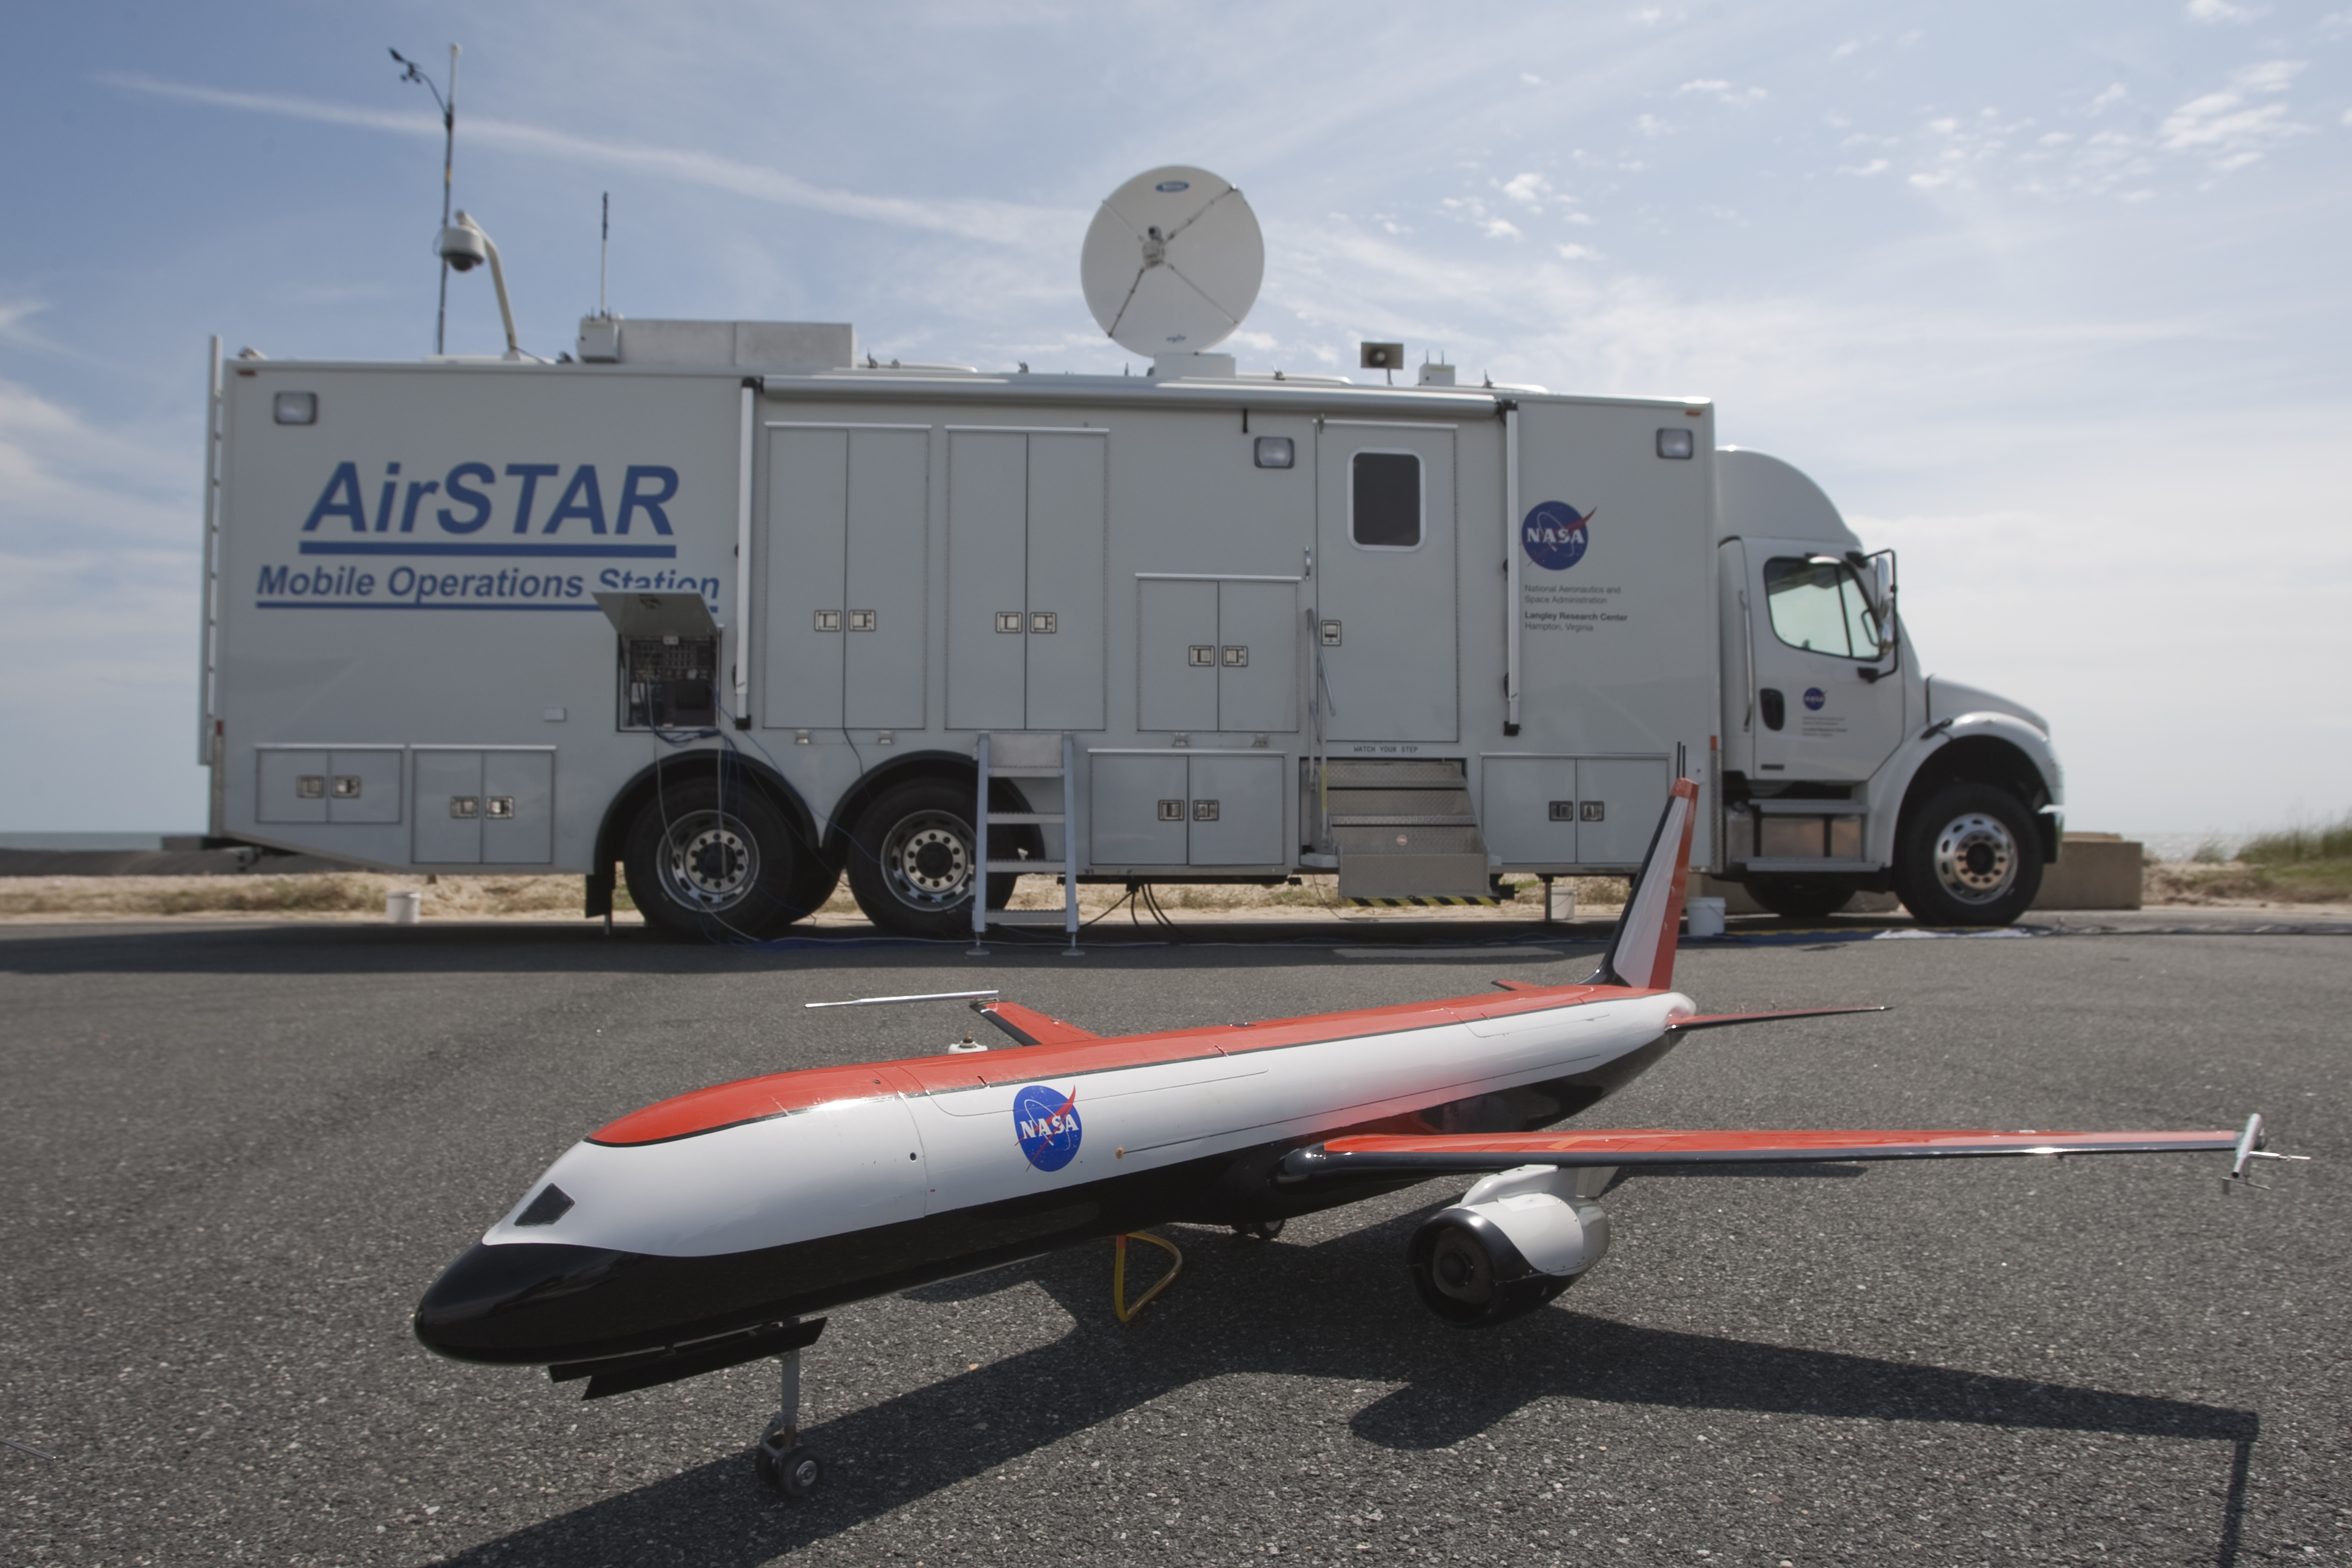
\includegraphics[width=3in]{airstar_0.jpg}
    \caption{GTM, image credit to NASA and Sean Smith \cite{airstar}}
    \label{fig:gtm}
\end{figure}

Chakraborty et al summarize the longitudinal dynamics of the GTM, based off of a simulink model and aerodynamic coefficient look-up tables provided by NASA \cite{primary}. No reference frames were provided, therefore for the purposes of this report it is assumed that all $x,y,z$ body axis are the traditionally defined longitudinal aircraft body axis: with the body frame centered at the vehicle's center of gravity, the body-$x$ axis points through the nose of the aircraft, the body-$y$ axis points over the right wing, and the body-$z$ axis points down below the vehicle \cite{body}.

\section{Original State Dynamics} 

An overview of system variables and constants can be found in \textbf{figure 2} and \textbf{figure 3}. The state dynamics are described with 4 states, and 2 inputs. The longitudinal state equations are provided in this section \cite{primary}.

$$ x = \begin{bmatrix} V \\ \alpha \\ q \\ \theta \end{bmatrix},\ \ u = \begin{bmatrix} \delta_{elev} \\ \delta_{th} \end{bmatrix} $$ 

\begin{align}     
        \dot{V} &= \frac{1}{m}\left(-D - m g \sin{(\theta - \alpha)} + T_x \cos{\alpha} + T_z \sin{\alpha} \right) \\
        \dot{\alpha} &= \frac{1}{m V}\left(-L + m g \cos{(\theta - \alpha)} - T_x \sin{\alpha} + T_z \cos{\alpha}\right) + q \\
        \dot{q} &= \frac{M + T_m}{Iyy} \\
        \dot{\theta} &= q
\end{align}

The aerodynamic and engine thrust thrust forces and moments are described by the equations below \cite{primary}. \\ \\
\textbf{Aerodynamic Terms:}

 \begin{align}
        \bar{q} &= \frac{1}{2} \rho V^2 \\ 
        \hat{q} &= \frac{\bar{c}}{2 V} q  \\ 
        D &= \bar{q}\, S\, C_D\, (\alpha, \delta_{elev}, \hat{q})  \\ 
        L &= \bar{q}\, S\, C_L\, (\alpha, \delta_{elev}, \hat{q})  \\ 
        M &= \bar{q}\, \bar{c}\, S\, C_m\, (\alpha, \delta_{elev}, \hat{q}) 
\end{align}


\textbf{Thrust Terms:}
\begin{align}
    T_x(\delta_{th}) &= n_{ENG} T(\delta_{th}) \cos{(\epsilon_2)} \cos{(\epsilon_3)} \\ 
    T_z(\delta_{th}) &= n_{ENG} T(\delta_{th}) \sin{(\epsilon_2)} \cos{(\epsilon_3)} \\ 
    T_m(\delta_{th}) & = r_z T_x(\delta_{th}) - r_x T_z(\delta_{th})
\end{align}

The dynamical equations (1-4) describe a sum of forces and torques that change the vehicle's air speed, angle of attack, pitch rate, and pitch angle. The engine thrust $T(\delta_{th})$ is a ninth-order polynomial, which was provided to Chakraborty et al by NASA \cite{primary}. At this point, the vehicle's model is well defined. While nonlinear analysis could be applied to these state dynamics as written, the proposed ROA estimation method uses SOS optimization methods, which requires dynamics in polynomial form. 

To allow SOS optimization methods to be used to estimate the ROA of asymptotically stable trim conditions, the dynamics listed above are approximated as low-order polynomials in the following section. Specifically, low angle of attack trim conditions were of interest. Therefore, the polynomial approximations developed were weighted to be most accurate for the prioritized low angle of attack trim conditions \cite{primary}. Higher order polynomials were approximated as lower order polynomials to reduce computional complexity; SOS optimizations are particularly sensitive to dynamical models with many states, and high-order dynamical models.

\begin{figure}
    \centering
    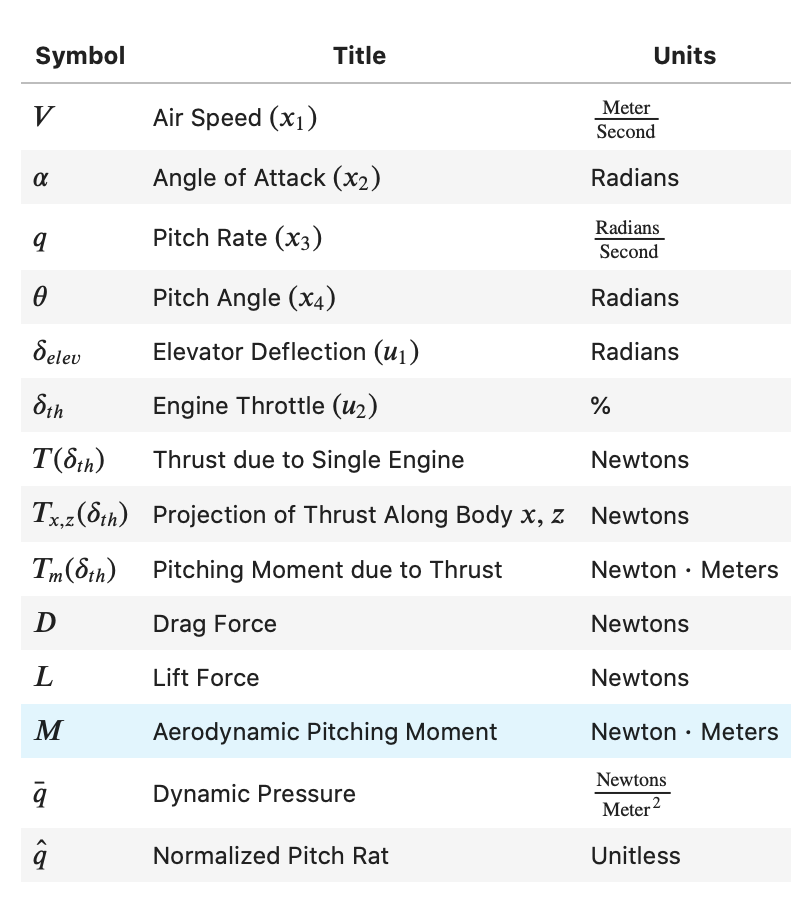
\includegraphics[width=3in]{variables.png}
    \caption{GTM Longitudinal Dynamics Variables}
    \label{fig:variables}
\end{figure}

\begin{figure}
    \centering
    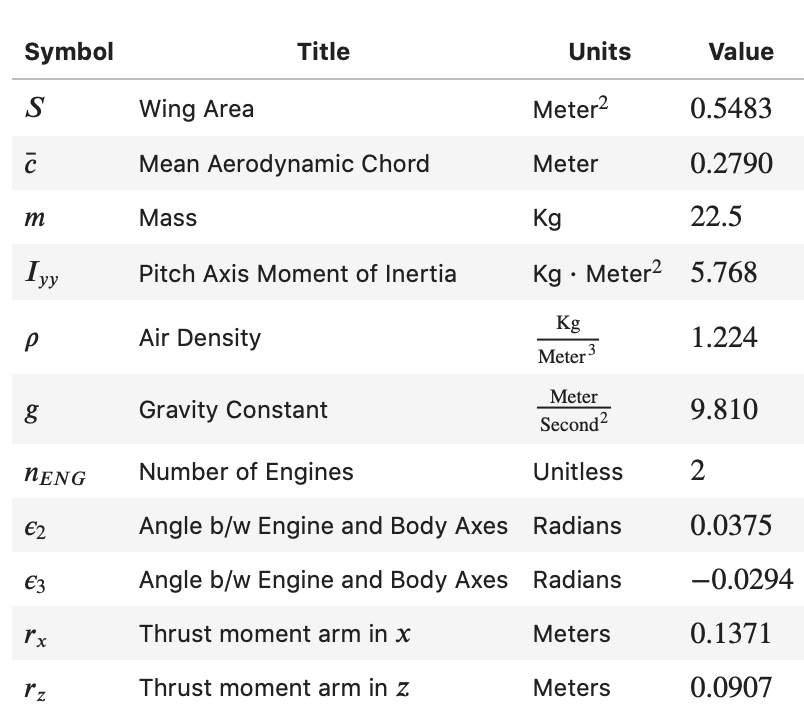
\includegraphics[width=3in]{constants.png}
    \caption{GTM Longitudinal Dynamics Constants}
    \label{fig:variables}
\end{figure}

\section{Polynomial Approximations}

The following dynamical terms are approximated by low-order polynomials \cite{primary}. Methods for approximating each term are described in this section. 

\begin{enumerate}
    \item Trigonometric functions: \\ $\sin{(\alpha)},\ \cos{(\alpha)}, \sin{(\theta - \alpha)},\ \cos{(\theta- \alpha)}$
    \item Engine model: $T(\delta_{th})$
    \item Rational dependence on speed: $\frac{1}{V}$
    \item Aerodynamic coefficients: $C_D,\ C_L,\ C_m$
\end{enumerate}

\subsection{Trigonometric Function}

Finding polynomial approximations for the $\sin$ and $\cos$ terms in the dynamics is relatively straightforward: Taylor Series expansions provide approximate polynomial forms for both trigonometric functions. By replacing each $\sin(z)$ and $\cos(z)$ term with the first two elements of their series expansions (shown below), Chakraborty et al found a maximum approximation error of $0.25\%$ for $\sin(z)$, and $2.2\%$
for $\cos(z)$ for $|z| \leq \frac{\pi}{4}$ \cite{primary}.

\begin{align*}
    \sin{(z)} & \approxeq z - \frac{z^3}{3!}  \ \ \ \text{ for } z \ \text{in Radians} \\
    & \implies \sin{(\alpha)} \approxeq \alpha - \frac{1}{6}\alpha^3 \tag{13} \\
    & \implies \sin{(\theta - \alpha)} \approxeq (\theta - \alpha) - \frac{1}{6}(\theta - \alpha)^3 \tag{14}
\end{align*}

\begin{align*}
    \cos{(z)} & \approxeq z - \frac{1}{2!} z^2  \ \ \ \text{ for } z \ \text{in Radians} \\
    & \implies \cos{(\alpha)} \approxeq \alpha - \frac{1}{2}\alpha^2 \tag{15} \\
    & \implies \cos{(\theta - \alpha)} \approxeq (\theta - \alpha) - \frac{1}{2}(\theta - \alpha)^2 \tag{16}
\end{align*}

\subsection{Engine Model}

As previously mentioned, a ninth-order polynomial engine model was provided by NASA \cite{primary}. Public GTM models are available \cite{sosopt}\cite{github}, but the exact ninth-order polynomial engine model was not found in time for this report. It may or may not be publicly available. The ninth-order engine polynomial model was approximated as a third order polynomial model, which only introduced a maximum approximation error of $1.3\%$ through the range of thrust inputs $\delta_{th} \in \left[ 0, 100 \right]$ \cite{primary}.

\begin{align*}
    T(\delta_{th}) \approxeq
        &- 8.751 \times 10^{-6} \delta_{th}^3 \\
        &+ 5.115 \times 10^{-3} \delta_{th}^2 \\
        &+ 3.673 \times 10^{-1} \delta_{th} 
        + 4.825 \tag{17}
\end{align*}

\subsection{Rational Dependence on Speed}

The $\frac{1}{V}$ terms can be approximated as a first order polynomial through curve fitting. Specifically, the least squares curve fitting method was applied to a set of air speeds between $30 \frac{m}{s}$ and $60 \frac{m}{s}$. This air speed range was chosen because the air speed trim condition discussed later in this document falls right in the center, at $45 \frac{m}{s}$ \cite{primary}. Chakraborty et al found a $9\%$ maximum error introduced with this polynomail approximation \cite{primary}. 

SciPy's \verb+curve_fit+ function was used to replicate the first order polynomial found by Chakraborty et al. The replicated first order polynomial approximation closely matched the published results \cite{primary}.

\begin{equation*}
    \frac{1}{V} \approxeq -5.304 \times 10^{-4} V + 4.699 \times 10^{-2} \tag{18}
\end{equation*}

\subsection{Aerodynamic Coefficients}
Aerodynamic coefficients $C_x, C_z, C_m$ were provided to Chakraborty et al by NASA via lookup tables, which were conditioned on $\alpha,\, \delta_{elev},\, \text{and}\, \hat{q} $ \cite{primary}. Rather than modify the drag force term $D$ by substituting $-D = D_x \cos\alpha + D_z \sin\alpha$, which would introduce additional approximation errors due to the trigonometric functions, the $C_x$ and $C_z$ look-up table data was first transformed into lift and drag coordinates \cite{primary}.

\begin{equation*}
    \begin{bmatrix} C_D \\ C_L \end{bmatrix} = -\begin{bmatrix} \cos\alpha & \sin\alpha \\ -\sin\alpha & \cos\alpha \end{bmatrix} \begin{bmatrix} C_x \\ C_z \end{bmatrix} \tag{19}
\end{equation*}

The look-up table data for $C_D, C_L, C_m$ was then approximated by polynomial expressions using a least squares curve fitting technique. The curve fitting for the aerodynamic coefficients was weighted to be most accurate for low angles of attack: $-5\deg \leq \alpha \leq 15\deg$ \cite{primary}. This allows the polynomial approximation to be most accurate for the level flight trim condition that will be analyzed in following sections. 

The look-up table data for the aerodynamic coefficients was provided as a sum of three terms. As a result, a polynomial approximation was produced for each of the terms. The following expression for $C_*$ is valid for $C_D,C_L,C_m$ \cite{primary}.

\begin{align*}
        C_*(\alpha, \delta_{elev}, \hat{q}) = 
        &C_{*,\alpha}(\alpha) \\
        &+ C_{*,\delta_{elev}}(\alpha, \delta_{elev}) \\
        &+ C_{*,\hat{q}}(\alpha,\hat{q}) \tag{20}
\end{align*}

The plot in \textbf{Figure 4} shows the look-up data for $C_{D,\alpha}, C_{L,\alpha}, C_{m,\alpha}$, and the corresponding curve fit for each (once again, weighted to be most accurate for low angles of attack) \cite{primary}. The polynomial expressions for each aerodynamic coefficient term are provided in this section \cite{primary}.

\begin{figure}
    \centering
    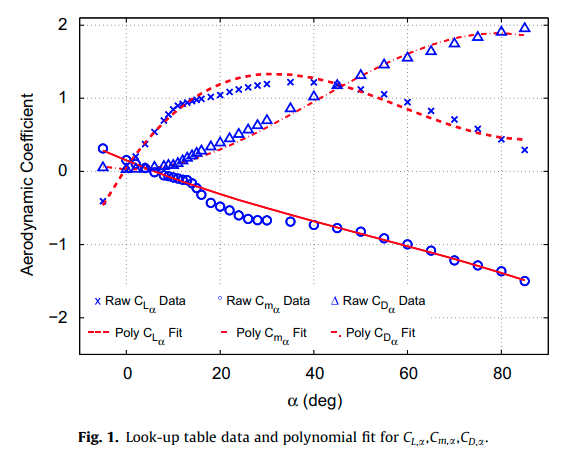
\includegraphics[width=3in]{fig1_published.png}
    \caption{Curve Fitting for $C_{D,\alpha}, C_{L,\alpha}, C_{m,\alpha}$ \cite{primary}}
    \label{fig:my_label}
\end{figure}

\begin{align*}
C_{D,\alpha}(\alpha) = &-1.477\alpha^3 + 3.110\alpha^2 - 1.303\times10^{-1}\alpha \\
&+ 3.060\times10^{-2} \\ 
C_{D,\delta_{elev}}(\alpha,\delta_{elev}) = &- 5.943\times10^{-2}\alpha^2 + 1.435\times10^{-1}\alpha\delta_{elev} \\
&+ 5.967\times10^{-2}\delta_{elev}^2 + 2.661\times10^{-2}\alpha \\
&+ 2.733\times10^{-2}\delta_{elev} - 1.903\times10^{-3} \\
C_{D,\hat{q}}(\alpha,\hat{q}) = &- 2.917\times10^{-2}\alpha^2 + 33.58\alpha\hat{q} - 151.0\hat{q}^2 \\
&- 3.022\times10^{-3}\alpha - 9.691\times10^{-1}\hat{q} \\
&+ 2.221\times10^{-4} \\ 
\star\ C_D(\alpha, \delta_{elev}, \hat{q}) = 
        &\ C_{D,\alpha}(\alpha) + C_{D,\delta_{elev}}(\alpha, \delta_{elev}) \tag{21} \\ 
        &+ C_{D,\hat{q}}(\alpha,\hat{q}) \\ 
\
C_{L,\alpha}(\alpha) = &+2.141\alpha^3 - 6.575\alpha^2 + 5.298\alpha \\
&+ 5.337\times10^{-2} \\
C_{L,\delta_{elev}}(\alpha,\delta_{elev}) = &+ 4.188\times10^{-3}\alpha^2 - 3.438\times10^{-1}\alpha\delta_{elev} \\
&+ 9.293\times10^{-2}\delta_{elev}^2 - 3.497\times10^{-2}\alpha  \\
&+ 4.610\times10^{-1}\delta_{elev} + 2.543\times10^{-3} \\
C_{L,\hat{q}}(\alpha,\hat{q}) = &+ 2.297\times10^{-2}\alpha^2 - 1.359\alpha\hat{q} - 856.7\hat{q}^2 \\
&- 1.673\times10^{-2}\alpha + 34.38\hat{q} + 3.703\times10^{-3} \\
\star\ C_L(\alpha, \delta_{elev}, \hat{q}) = 
        &\ C_{L,\alpha}(\alpha) + C_{L,\delta_{elev}}(\alpha, \delta_{elev}) \tag{22} \\ 
        &+ C_{L,\hat{q}}(\alpha,\hat{q}) \\
\
C_{m,\alpha}(\alpha) = &- 2.199\times10^{-1}\alpha^3 + 5.912\times10^{-1}\alpha^2 \\
&+ 1.498\alpha + 1.516\times10^{-1} \\
C_{m,\delta_{elev}}(\alpha,\delta_{elev}) = &+1.263\alpha\delta_{elev} - 1.887\delta_{elev} \\
C_{m,\hat{q}}(\alpha,\hat{q}) = &-41.24\hat{q} \\
\star\ C_m(\alpha, \delta_{elev}, \hat{q}) = 
        &\ C_{m,\alpha}(\alpha) + C_{m,\delta_{elev}}(\alpha, \delta_{elev}) \tag{23} \\ 
        &+ C_{m,\hat{q}}(\alpha,\hat{q}) \\ 
\end{align*}

\subsection{Final Polynomial Model}
The final polynomial model derived by Chakraborty et al follows \cite{primary}. This model was implemented (read, explicitly typed from \cite{primary}) as Python code for this report. An attempt was made to construct the polynomial model by substituting the previous polynomial terms into the original state equation. While this resulted in polynomial dynamics, the constructed dynamics did not seem to match completely with the published results, and they caused the simulation time to spike to an extremly long run time (while the hard-coded published dynamics could be simulated in a minute or two). As a result, the published polynomial model was included in this report, and was used for all simulation and analysis.

$$ \dot{x} = \begin{bmatrix} V \\ \alpha \\ q \\ \theta \end{bmatrix} = \begin{bmatrix} f_1(x,u) \\ f_2(x,u) \\ f_3(x,u) \\ f_4(x,u) \end{bmatrix},\ u = \begin{bmatrix} \delta_{elev} \\ \delta_{th} \end{bmatrix} $$ 
\begin{align*}
f_1(x,u) = \
&\ 1.233\times10^{-8}x_1^4x_3^2 + 4.853\times10^{-9}x_2^3u_2^3 \\
&+ 3.705\times10^{-5}x_1^3x_2 x_3 
- 2.184\times10^{-6}x_1^3x_3^2 \\
&+ 2.203\times10^{-2}x_1^2x_2^3 - 2.836\times10^{-6}x_2^3u_2^2 \\
& + 3.885\times10^{-7}x_2^2u_2^3 - 1.069\times10^{-6}x_1^3x_3 \\
& - 4.517\times10^{-2}x_1^2x_2^2
- 2.140\times10^{-3}x_1^2x_2u_1 \\
&- 3.282\times10^{-3}x_1^2x_2 x_3 - 8.901\times10^{-4}x_1^2u_1^2 \\
& + 9.677\times10^{-5}x_1^2x_3^2 - 2.037\times10^{-4}x_2^3u_2 \\
&- 2.270\times10^{-4}x_2^2u_2^2
- 2.912\times10^{-8}x_2u_2^3 \\
&+ 1.591\times10^{-3}x_1^2x_2 - 4.077\times10^{-4}x_1^2u_1 \\
& + 9.475\times10^{-5}x_1^2x_3 - 1.637x_2^3 \\
&- 1.631\times10^{-2}x_2^2u_2 + 4.903x_2^2x_4 \\
& -4.903x_2x_4^2 + 1.702\times10^{-5}x_2u_2^2 \\
&- 7.771\times10^{-7}u_2^3 + 1.634x_4^3  \\
&- 4.319\times10^{-4}x_1^2 - 2.142\times10^{-1}x_2^2 \\
&+ 1.222\times10^{-3}x_2u_2
+ 4.541\times10^{-4}u_2^2 \\
&+ 9.823x_2 + 3.261\times10^{-2}u_2 \\
&- 9.807x_4 + 4.282\times10^{-1}
\tag{24}
\end{align*}

\begin{align*}
f_3(x,u) = \
\
& - 6.573\times10^{-9}x_1^5x_3^3 + 1.747\times10^{-6}x_1^4x_3^3 \\
&- 1.548\times10^{-4}x_1^3x_3^3 
\
- 3.569\times10^{-3}x_1^2x_2^3 \\
&+ 4.571\times10^{-3}x_1^2x_3^3 + 4.953\times10^{-5}x_1^3x_3 \\
\
& + 9.596\times10^{-3}x_1^2x_2^2 + 2.049\times10^{-2}x_1^2x_2u_1 \\
&- 2.431\times10^{-2}x_1^2x_2 
\
- 3.063\times10^{-2}x_1^2u_1 \\
&- 4.388\times10^{-3}x_1^2x_3 - 2.594\times10^{-7}u_2^3 \\
\
& + 2.461\times10^{-3}x_1^2 + 1.516\times10^{-4}u_2^2 \\
&+ 1.089\times10^{-2}u_2 + 1.430\times10^{-1}
\tag{26}
\end{align*}

\begin{align*}
f_2(x,u) = \
& -3.709\times10^{-11}x_1^5x_3^2 + 6.869\times10^{-11}x_1x_2^3u_2^3 \\
&+ 7.957\times10^{-10}x_1^4x_2 x_3 
+ 9.860\times10^{-9}x_1^4x_3^2 \\
&+ 1.694\times10^{-5}x_1^3x_2^3 - 4.015\times10^{-8}x_1x_2^3u_2^2 \\
\
& - 7.722\times10^{-12}x_1x_2^2u_2^3 - 6.086\times10^{-9}x_2^3u_2^3 \\
&- 2.013\times10^{-8}x_1^4x_3
\
- 5.180\times10^{-5}x_1^3x_2^2 \\
&- 2.720\times10^{-6}x_1^3x_2u_1 
- 1.410\times10^{-7}x_1^3x_2 x_3 \\
\
& + 7.352\times10^{-7}x_1^3u_1^2 - 8.736\times10^{-7}x_1^3x_3^2 \\
&- 1.501\times10^{-3}x_1^2x_2^3 
\
- 2.883\times10^{-6}x_1x_2^3u_2 \\
&+ 4.513\times10^{-9}x_1x_2^2u_2^2 - 4.121\times10^{-10}x_1x_2u_2^3 \\
\
& + 3.557\times10^{-6}x_2^3u_2^2 + 6.841\times10^{-10}x_2^2u_2^3 \\
&+ 4.151\times10^{-5}x_1^3x_2 + 3.648\times10^{-6}x_1^3u_1 \\
&+ 3.566\times10^{-6}x_1^3x_3 
+ 6.246\times10^{-6}x_1^2x_2 x_3 
\\
& + 4.589\times10^{-3}x_1^2x_2^2 + 2.410\times10^{-74}x_1^2x_2u_1 \\
&- 6.514\times10^{-5}x_1^2u_1^2 
\
+ 2.580\times10^{-5}x_1^2x_3^2 \\
&- 3.787\times10^{-5}x_1x_2^3 + 3.241\times10^{-7}x_1x_2^2u_2 \\
\
& + 2.409\times10^{-7}x_1x_2u_2^2 + 1.544\times10^{-11}x_1u_2^3 \\
&+ 2.554\times10^{-4}x_2^3u_2 
\
- 3.998\times10^{-7}x_2^2u_2^2 \\
&+ 3.651\times10^{-8}x_2u_2^3 + 4.716\times10^{-7}x_1^3 \\
\
& - 3.677\times10^{-3}x_1^2x_2 - 3.231\times10^{-4}x_1^2u_1 \\
&- 1.579\times10^{-4}x_1^2x_3 
\
+ 2.605\times10^{-3}x_1x_2^2 \\
&+ 1.730\times10^{-5}x_1x_2u_2 
- 5.201\times10^{-3}x_1x_2x_4 \\
\
&- 9.026\times10^{-9}x_1u_2^2 
+ 2.601\times10^{-3}x_1x_4^2 \\
&+ 3.355\times10^{-3}x_2^3 
\
- 2.872\times10^{-5}x_2^2u_2 \\
&- 2.134\times10^{-5}x_2u_2^2 
- 1.368\times10^{-9}u_2^3 \\
\
 &- 4.178\times10^{-5}x_1^2 
 + 2.272\times10^{-4}x_1x_2 \\
 &- 6.483\times10^{-7}x_1u_2 
\
- 2.308\times10^{-1}x_2^2 \\
&- 1.532\times10^{-3}x_2u_2 
+ 4.608\times10^{-1}x_2x_4 \\
\
&- 2.304\times10^{-1}x_4^2 
+ 7.997\times10^{-7}u_2^2 \\
&- 5.210\times10^{-3}x_1  - 2.013\times10^{-2}x_2 \\
&+ 5.744\times10^{-5}u_2 + x_3 
+ 4.616\times10^{-1} \tag{25}
\
\end{align*}

\begin{align*}
    f_4(x,u) = x_3 \tag{27}
\end{align*}

\newpage
\section{Analysis}

\subsection{Trim Condition}

The longitudinal polynomial dynamics were analyzed near the following level-flight trim condition \cite{primary}. For this report, the trim condition was verified to cause $f(x_t,u_t)$ to be close to zero. 

\begin{equation*}
    x_t = 
        \begin{bmatrix} 
            x_{1,t} \\ x_{2,t} \\ x_{3,t} \\ x_{4,t} 
        \end{bmatrix} = 
        \begin{bmatrix} 
            V_t \\ \alpha_t \\ q_t \\ \theta_t 
        \end{bmatrix} = 
        \begin{bmatrix}
            45\ \  \text{m/s} \\
            0.04924\ \  \text{rad} \\
            0\ \  \text{rad/s} \\
            0.04924\ \  \text{rad}
        \end{bmatrix} \tag{27}
\end{equation*}

\begin{equation*}
        u_t = 
        \begin{bmatrix}
            u_{1,t} \\ u_{2,t}
        \end{bmatrix} = 
        \begin{bmatrix}
            \delta_{elev,t} \\
            \delta_{th,t}
        \end{bmatrix} = 
        \begin{bmatrix}
            0.04892\ \  \text{rad} \\
            14.33\ \  \text{\%}
        \end{bmatrix} \tag{28}
\end{equation*}

Lyapunov's Indirect Method can be used to show that this trim condition is asymptotically stable for both the linearized and nonlinear dynamics. As shown below, the eigenvalues of the linearized dynamics fall within the left half of the complex plane, therefore this trim condition is asymptotically stable. 

\begin{align*}
    A_t &= \frac{\partial f}{\partial x}|_{x=x_t,\ u=u_t} \\
    & \implies \text{eig}(A_t) = 
        \begin{bmatrix}
            -3.819 - 6.444 i
            \\-3.819 + 6.444 i \\-0.0181 - 0.267 i \\ -0.0181 + 0.267 i
        \end{bmatrix} \tag{29}
\end{align*}

\subsection{Decoupled Modal Oscillations}

Before continuing to ROA analysis, recall that the computational expense of SOS optimization algorithms is very sensitive to the number of states, and the degree of the polynomial models \cite{primary}. The computational complexity for estimating this trim condition's ROA can be reduced if the number of states, and the degree of the polynomial models can be lowered. The eigenvalues of the linearized dynamics about the trim condition show two modal oscillations. Indeed, the nonlinear dynamics about this trim condition feature a slower phugoid oscillation involving $x_1,\ x_4,$ and $u_2$, and a faster short-period oscillation involving $x_2, x_3,$ and $u_1$\cite{primary}. These two oscillations are in fact coupled, but they can be sufficiently approximated as decoupled by holding less relevant states and inputs at their trim conditions. The following approximation for the decoupled short period mode, $g(x_2,x_3,u_1)$, can be defined.

\begin{equation*}
    g(x_2,x_3,u_1) = \begin{bmatrix} f_2(x_{1,t}, x_2, x_3, x_{4,t}, u_1, u_{2,t}) \\ f_3(x_{1,t}, x_2, x_3, x_{4,t}, u_1, u_{2,t}) \end{bmatrix} \tag{30}
\end{equation*} \\

By decoupling the nonlinear short period modal oscillations, the region of attraction for the nonlinear short period oscillation about this trim condition can be estimated, in addition to estimating the region of attraction for the 4-state dynamics about this trim condition. Estimating the ROA of the 2-state approximated, decoupled, nonlinear short-period mode will be a computationally easier task due to the lower number of states. As a result, estimating the ROA for the decoupled short period mode would take less computation time than estimating the ROA for the complete polynomial dynamics about this trim condition \cite{primary}.

Simulating the nonlinear decoupled short period dynamics alongside the complete nonlinear polynomial dynamics (with the same few test initial conditions, all inputs held at trim, and $x_1$ and $x_4$ held at trim in the 4-state simulation) gives confidence that the approximation technique for decoupling the nonlinear short period mode is valid. This result was replicated for the purpose of this report. The complete polynomial short period dynamics were plotted in dashed, colored lines, while the decoupled short period dynamics were plotted in solid black lines. Both the replicated and published results show a good match. The authors note that the decoupled short period dynamics converge to the trim condition, while the complete polynomial dynamics have different behavior very close to the trim condition. This is a consequence of the phugoid mode, which causes slow oscillations near the trim condition \cite{primary}. The simulation results, which show the trim condition to be a stable focus, are in \textbf{Figure 5}. 

\begin{figure*}
    \centering
    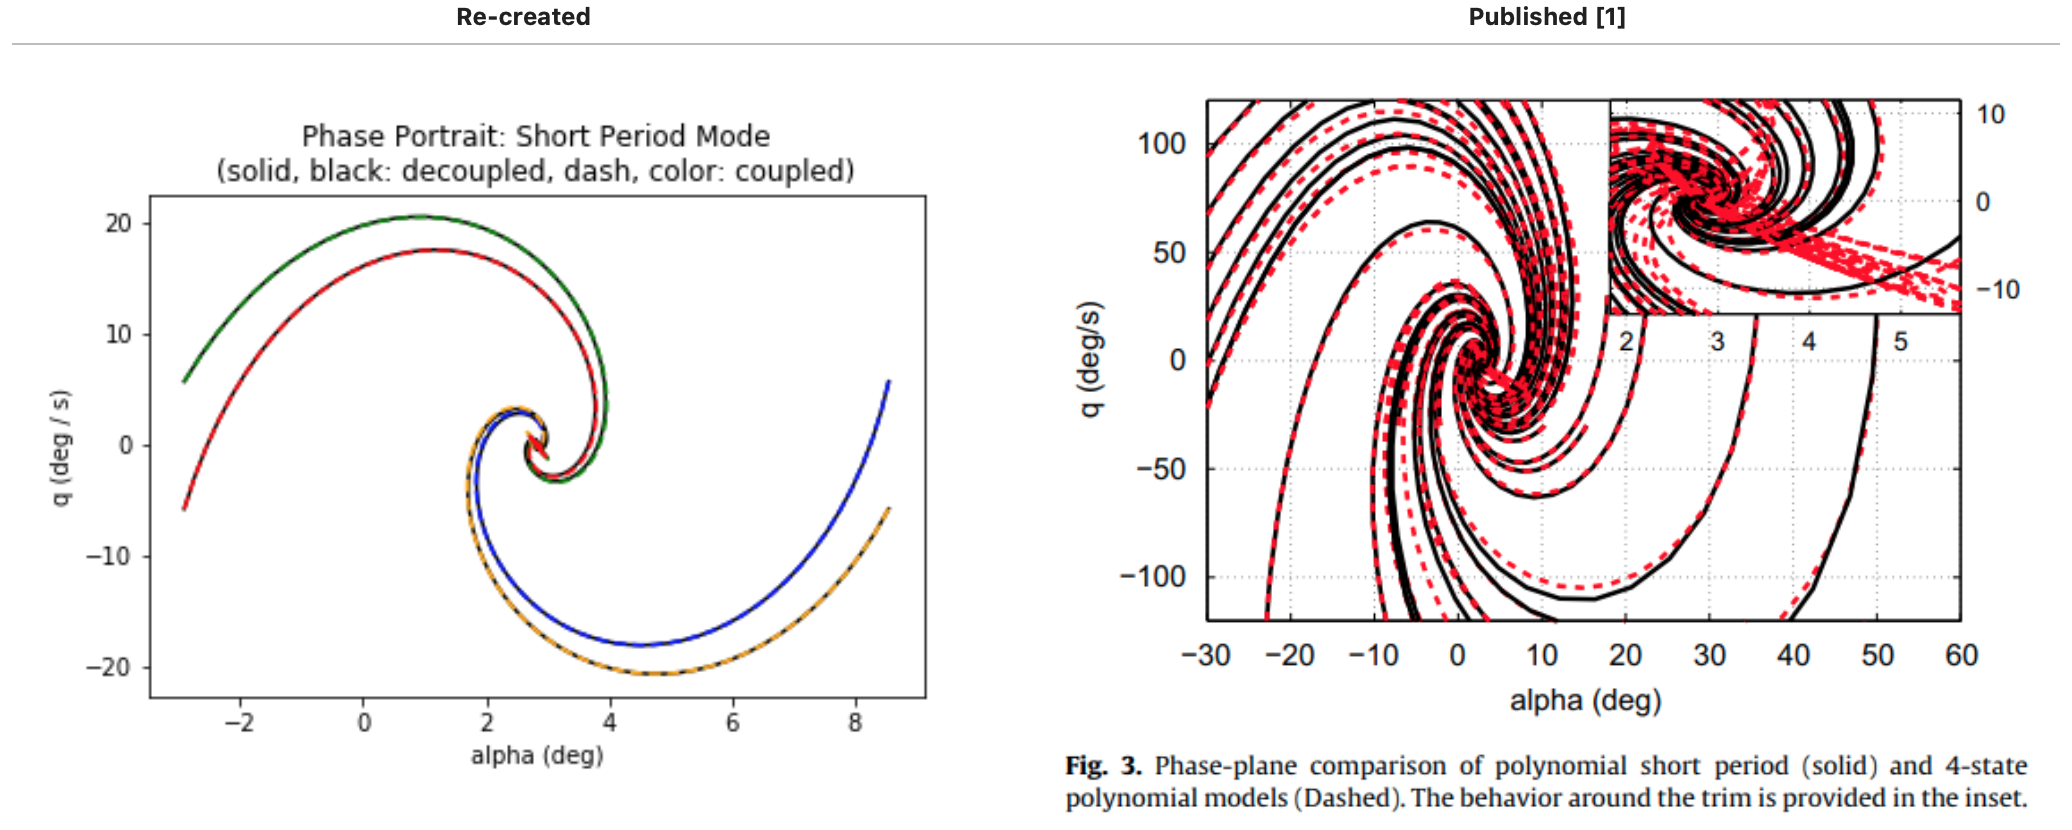
\includegraphics[height=3in]{comparison.png}
    \caption{Phase Portrait for Short Period Mode: replicated (left), published (right)}
    \label{fig:comparison}
\end{figure*}

\subsection{Proof the ROA is not $\mathbb{R}^n$}

As shown in \textbf{Figure 6}, there exists an initial condition which causes the state to diverge from the trim condition. The initial conditions for the replicated plot in \textbf{Figure 5} were $\pm0.1$ perturbations off of the short period states $x_2$ and $x_3$. The initial conditions in \textbf{Figure 6} were $\pm0.5$ perturbations off of the short period states. This small change resulted in three divergant trajectories. Therefore, the trim condition is not globally asymptotically stable, and the region of attraction for this trim condition is not $\mathbb{R}^n$.

\begin{figure}
    \centering
    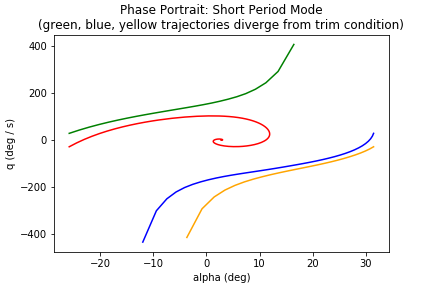
\includegraphics[width=3.6in]{fig3_redo_divergent.png}
    \caption{Divergent Short Period Trajectories}
    \label{fig:my_label}
\end{figure}

\subsection{ROA Estimation Setup}

As previously mentioned, searching the the precise ROA for an aysmptotically stable trim condition is very difficult. Instead, Chakraborty et al propose searching for upper and lower bounds for an ellipsoidal invariant subset of the ROA. They note that, if the upper and lower bounds are close, then for practical purposes the ROA has been well estimated \cite{primary}. 

The authors limited the search to ellipsoidal subsets of the ROA. As a result, two definitions will need to be introduced to properly quantify the ellipsoids. First, the "shape function" $p(z) = z^T N z$ for some $n \times n$ symmetric matrix $N$ is defined \cite{primary}. Second, the "level set" or "ellipsoid" $\epsilon_\beta = \{ z \in \mathcal{R}^n : p(z) \leq \beta \}$ is defined \cite{primary}. The authors state: 

\begin{quote}
"The choice of $p(x)$ is problem dependent and reflects dimensional scaling information, as well as the importance of certain directions in the state space. Given the shape function $p(x)$, the problem is to find the largest ellipsoid $\epsilon_\beta$ contained in the ROA" \cite{primary}.
\end{quote}

Here, the ellipsoid is $\epsilon_\beta$, the shape of the ellipse is $p(x)$, and the size of the ellipse is $\beta$. Finding the largest ellipsoid $\epsilon_\beta$ in the ROA in equivalent to finding $\beta^*$ such that $\beta^* = \text{max}\beta\ \text{ subject to: }\ \epsilon_\beta \subset \mathcal{R}$, where $\mathcal{R}$ is the ROA of the trim condition \cite{primary}. Finding the largest ellipsoid is still a difficult task, so Chakrabory et al propose solving for upper and lower bounds on the ROA estimate. 

\subsubsection{Upper Bound Methodology}
An upper bound for the trim condition's ROA estimate can be found by running high-fidelity simulations, and searching for divergent trajectories. The algorithm, as published by Chakraborty et al, follows \cite{primary}. First, guess at a large size $\beta_{try}$ of the upper bound ellipsoidal subset of the ROA. Next, choose random initial conditions on the boundary of the ellipse $\epsilon_\beta_{try}$, and simulate the dynamics from that initial condition. Once a divergent trajectory is found, reduce the $\beta_{try}$ value by a set factor (the authors chose $0.995$), and continue the algorithm until the desired amount of iterations is reached \cite{primary}. Written mathematically... \cite{primary}

\begin{enumerate}
    \item Guess at a large ROA ellipsoid size $\beta_{try}$
    \item Choose random initial conditions $x_0$ that satisfy $p(x_0)=\beta_{try}$, then simulate the dynamics from that initial condition. Keep picking initial conditions that satisfy $p(x_0)=\beta_{try}$ until a divergent trajctory is found (or the maximum number of iterations is reached)
    \item If the initial condition causes a divergent trajectory, reduce $\beta_{try}$ by a factor of $0.995$, and repeat the algorithm
    \item Repeat until the desired number of algorithm iterations is reached. Define the final value the upper bound $\overline{\beta}$ for the ellipsoidal invariant subset within the ROA.
\end{enumerate} 

\subsubsection{Lower Bound Methodology}
Chakraborty et al describe how Lyapunov theory can be used to find lower bounds for invariant ellipsoidal subsets of the trim condition's ROA. \textbf{Figure 7} is a lemma that was published in \cite{primary}, and potentially referenced from \cite{lemma}. This concept is familiar from ENAE 743's curriculum. The intersection of the region of state space where the Lyapunov function is bounded with the region of state space where the divergence of the Lyapunov function is negative definite is an invariant subspace of the region of attraction. Note that this requires the origin to be asymptotically stable, and therefore the system can be transformed to move the trim condition to the origin \cite{primary}.

\begin{figure}
    \centering
    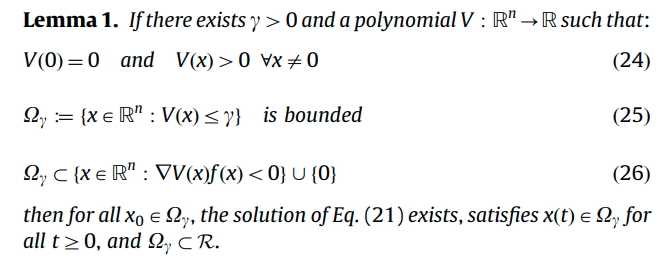
\includegraphics[width=3in]{lemma1.png}
    \caption{Lyapunov Theory applied to ROA Estimation \cite{primary}\cite{lemma}}
    \label{fig:lemma_labell}
\end{figure}

Because the origin of the (transformed) system is asymptotically stable, a Lyapunov function can be found by linearizing the zero-input dynamics about the origin, and solving the Lyapunov equation $A^T P + P A = -I$. Given $P>0$ that satisfies the Lyapunov equation, a Lyapunov function $V_{LIN}$ can be defined: $V_{LIN} = x^T P x$ \cite{primary}.

Given a Lyapunov function, the lower bound of the ellipsoidal ROA approximation can be found by "solving two maximizations": (31) and (32) \cite{primary}.

\begin{align*}
    \gamma^* &:= \text{max}\gamma \\
    &\ \ \ \ \text{ subject to: } \Omega_\gamma \subset \{ z \in \mathbb{R}^n : \Delta V(z)f(z) < 0 \} \tag{31} \\ \\
    \underline{\beta} &:= \text{max}\beta \\
    &\ \ \ \ \text{ subject to: } \ \epsilon_\beta \subset \Omega_\gamma \tag{32}
\end{align*}

Rather than directly maximize the second constraint, a sufficient condition is maximized (33) \cite{primary}. A polynomial which can be decomposed as a sum of squared terms, i.e. "$h = g_1^2 + g_2^2 + ... + g_n^2$", is defined a sum-of-squares (SOS) \cite{primary}.

\begin{align*}
     \underline{\beta} &:= \text{max}\beta \text{ subject to } \ s(z) \ \text{ is SOS, and } \\ 
     &\ \ \ \ -(\beta - p(z)s(z) + (\gamma^* - V(z)) \ \text{ is SOS } \tag{33}
\end{align*}

Replacing (32) with this sufficient condition transforms the lower bound ROA estimation task from a general constrained optimization problem, to a sum-of-squares constrained optimization problem. This is beneficial because sum-of-squares optimization problems have been researched, and software tools exist which can solve them \cite{primary}\cite{sosopt}\cite{sostools}. In (32), $s(x)$ is a "decision variable... found as part of the optimization" \cite{primary}. 

By taking advantage of existing SOS optimization tools, this sufficient condition can be solved more efficiently, and the lower bound $\underline{\beta}$ for an invariant ellipsoidal subset of the trim condition's ROA can be found.

If the lower bound and upper bound are close together, then the approximate maximum ellipsoidal subset of the ROA has practically been found \cite{primary}. Typically, the size of the lower bound ellipsoid $\underline{\beta}$ produced by the Lyapunov function $V_{LIN}$ is much smaller than the previously found upper bound \cite{primary}. To remedy this, a \textit{better} Lyapunov function must be chosen. An algorithm called $V$-$s$ iterations can iteratively bootstrap $V_{LIN}$ into a better Lyapunov function, which yields a larger lower bound $\underline{\beta}$. \textbf{Figure 8} describes the algorithm in more detail, with $l_1 (z) = -\epsilon_1 z^t z$ and $l_2(z) = -\epsilon_2 z^t z, for \epsilon_1,\ \epsilon_2 \approxeq 10^{-6}$ \cite{primary}.

\begin{figure}
    \centering
    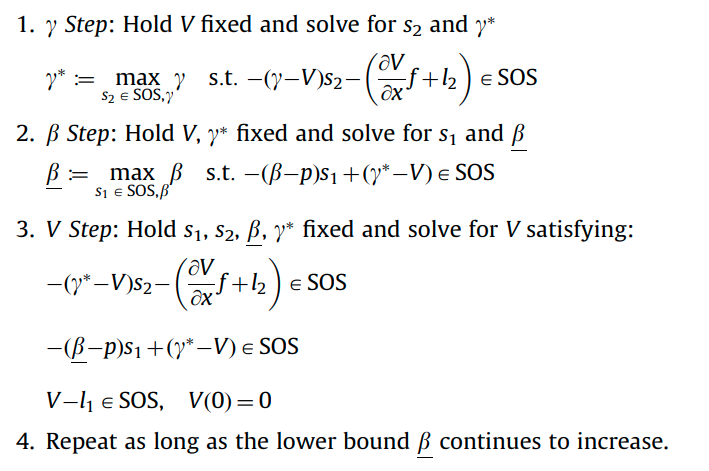
\includegraphics[width=3in]{vs_steps.png}
    \caption{Explanation of $V$-$s$ algorithm \cite{primary}}
    \label{fig:vs}
\end{figure}

Chakraborty et al found that calculating close lower and upper ROA bounds for the 2-state decoupled short period mode was much more computationally efficient than calculating lower and upper ROA bounds for the 4-state longitudinal polynomial dynamics. With a quartic Lyapunov function, the 2-state dynamics resulted in a lower bound $\underline{\beta} = 1.760$ in $0.02690$ hours \cite{primary}. The authors were also interested in the 4-state ROS estimate. They found the 4-state dynamics resulted in a larger $\underline{\beta}$ value of $3.360$, which was completed in $3.647$ hours \cite{primary}. This large difference in lower bound $\underline{\beta}$ is critical. The lower bound $\underline{\beta}$ can be viewed as a guaranteed invariant subset of the trim condition's true (and unknown) region of attraction. Therefore, the control engineers have confidence that any initial condition within the ellipsoid of size $\underline{\beta}$ will be driven back to the trim condition \cite{primary}. The results from Chakraborty et al's 4-state ROA estimation are presented in the next subsection.

\begin{figure*}
    \centering
    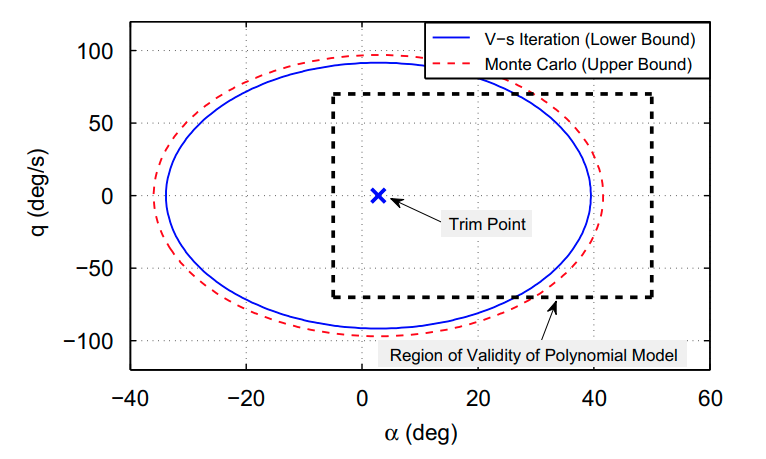
\includegraphics[width=5in]{final_roa.png}
    \caption{Ellipsoidal ROA bounds for 4-state polynomial dynamics \cite{primary}}
    \label{fig:final}
\end{figure*}

\subsection{4-state ROA Estimation}

Two more slight modifications can be made to the polynomial 4-state dynamics to simplify the ROA estimation calculations. Recall, once more, that the SOS optimization techniques that will be used for ROA estimation are computationally sensitive to the number of states, and the order of the polynomial. To simplify computations, polynomial terms with degree greater than 5, and/or coefficients less that $10^{-6}$ were removed. \cite{primary}. In addition, it was previously mentioned that the system would have to be transformed such that the origin of the system was asymptotically stable. The following transform, which applied to shift the trim condition to the origin, describes this more formally \cite{primary}.

\begin{equation*}
    z = \begin{bmatrix}
    z_1 \\ z_2 \\ z_3 \\ z_4 
    \end{bmatrix} = x - x_t = \begin{bmatrix}
    V-V_t \\ \alpha - \alpha_t \\ q - q_t \\ \theta - \theta_t
    \end{bmatrix}
\end{equation*}
    
The resulting ellipsoidal upper and lower bounds, as found by Chakraborty et al, for the trim condition's region of attraction are shown in \textbf{Figure 9} \cite{primary}. Note that the lower and upper bounds are quite close to one another; this gives confidence that there is not a much larger lower bound which could have been found, and as a result provided even more perturbation robustness guarantees. 

Recall the polynomial model approximations made in section IV introduced errors, and were tailored to low angle of attack flight conditions, as well as other state space operation assumptions \cite{primary}. The dotted box in \textbf{Figure 9} shows the region of short period state space where the polynomial model is accurate to the system \cite{primary}. Note that this region does not fill the entire ellipsoidal ROA approximation. 
\section{Conclusion}

The result shown in \textbf{Figure 9} is exciting, and modest simultaneously. Choosing Lyapunov functions often can be arbitrary. An exciting application within \cite{primary} is the use of $V$-$s$ iterations to find a better Lyapunov function, and as a result a larger invariant subset of the trim condition's region of attraction. At the same time, this report's introduction noted the potential shortcomings of relying on high-fidelity simulations \cite{primary}\cite{leaf}. Substantial work had to be done to come to the result in \textbf{Figure 9}, and the approximations did not allow full use of the ellipsoidal ROA estimate. Furthermore, this analysis was only for a single level-flight trim condition. 

As a student, the nonlinear analysis presented in \cite{primary} shows exciting methods and results, and also some clarity on why the aerospace industry largely uses linear analysis and high-fidelity simulations to validate flight control laws. Nonlinear analysis requires substantially more system-specific work than linear analysis; using general optimization and software analysis tools may require substantially transforming, or approximating, the dynamical model. Despite this, nonlinear analysis is important, as linear analysis and simulations can miss key dynamical elements \cite{primary}\cite{leaf}. The benefit from a high confidence ROA estimate is clear; a region of state space guaranteed to act robustly to perturbations is a powerful result.

\nocite{*}

\bibliography{apssamp}% Produces the bibliography via BibTeX.

\end{document}
%
% ****** End of file apssamp.tex ******
